
This chapter describes basic setup of the OpenTTP reference  platform, verification of its operation and logging in to the unit.

Warning !
The  unit contains a computer. This must be shut down properly
before power is removed from the unit. Failure to do this can 
result in inoperability of the system.
\marginpar{
\epsfig{file=figures/warning.eps,silent=,width=48pt}}
The system can be shut down from the front panel (\ref{sKeypad}) or by
logging in (\ref{sLoggingIn}).


\section{The front panel \label{sFrontPanel}}

\begin{figure}[h]
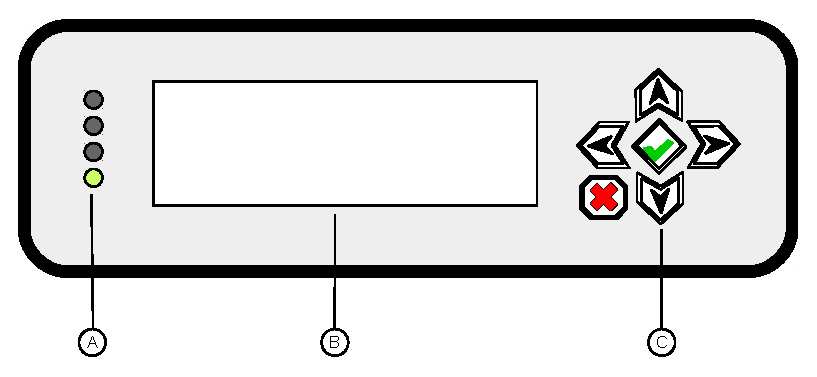
\psfig{file=figures/frontpanel.eps,silent=}
\caption{Front panel of the unit}
\end{figure}

\begin{itemize}
	\item[\mykey{A}] Status LEDs
	\item[\mykey{B}] LCD display
	\item[\mykey{C}] Keypad
\end{itemize}

The top line of the LCD display shows UTC date and time.
The date and time displayed will typically only be accurate to 1 s.
The contents of the second and third lines of the display depend on the display mode
\ref{ss:DisplayMode}.

The bottom line is reserved for notification of system alarms and either shows
`System OK' or `System Alarm'.
The adjacent LED will be red if there is a running alarm.
The other LEDs are currently unused.

\subsection{Using the front panel keypad \label{sKeypad} }

The keypad provides access to status information and limited control and configuration of the unit. 
It can be used to cleanly shut down or reboot the computer without logging in. 

System status is normally displayed on the screen.  
The menus are accessed by pressing any key. Menus are navigated  using the keypad:\\
%%\begin{table}[h]
\begin{tabular}{ll}
 \mykey{\begin{turn}{270}\ding{228}\end{turn}}& Move to next menu item \\
 \mykey{\begin{turn}{90}\ding{228}\end{turn}} & Move to previous menu item \\
 \mykey{\ding{228}}, \mykey{\ding{52}}& Select menu item \\
 \mykey{\begin{turn}{180}\ding{228}\end{turn}}  &Back to previous menu \\
 \mykey{\ding{54}}  & Back to the status display
\end{tabular}
%%\end{table}
\\
Escaping back to the status page after making a change will not undo the change.
Where a sub-menu lists a number of options, the currently selected option is flagged with an asterisk.

Dialogs are navigated using the cursor keys. A dialog will typically consist of a number of input fields.
Some of these work like buttons and are selected using the \mykey{\ding{52}} key; others may require inputting
a value and this is done by cycling through the possible values with the cursor keys.

If you move out of an input field, focus will pass to the next valid input field.

You can quit a dialog using the \mykey{\ding{54}} key. Any changes made in a dialog will not be applied if you quit it.

If a menu or dialog has been inactive for more than 5 minutes, the display returns
to showing system status.

\subsection{Menus}

The menu structure is shown below:

\begin{figure}[h]
\dirtree{%
 .1 Home screen.
 .2 Setup.
 .3 LCD setup.
 .4 LCD settings.
 .4 LCD backlight time.
 .3 Display mode.
 .4 GPS.
 .4 NTP.
 .4 GPSDO.
 .3 Show IP addresses.
 .2 Show alarms.
 .2 Show system info.
 .2 Restart.
 .3 GPS.
 .3 NTPD.
 .3 Reboot.
 .3 Power down.
}
\caption{Menu structure}
\end{figure}

\subsubsection{LCD setup}

The intensity and contrast of the LCD display can be set using this menu.
A timeout can also be set on the backlight.

\subsubsection{Display mode \label{ss:DisplayMode}}

The status information displayed by the unit in the second and third lines of the LCD display
can be selected as relating to either GPS, NTP or the GPSDO.

When in GPS mode, the identifiers of up
to 10 currently visible GPS space vehicles are displayed. 

When in NTP mode, the second line shows
the number of NTP packets received per minute. The third line shows information about
synchronization status, including leap second announcements.

In GPSDO mode, the second line shows whether the GPSDO is locked or not. 
The third line alternates between the `health' byte (\ref{sGPSDO}), and the estimated fractional frequency error 
(reported by the GPSDO) and the electronic frequency control (EFC) voltage, normalized to a maximum of 100.

\subsubsection{Show alarms}

This shows any currently running alarms as listed in \cc{/home/cvgps/logs/alarms}.

\subsubsection{Show system info}

This displays version and serial number information and the make of the installed oscillator.
This information is read from the file \cc{/usr/local/etc/sysinfo.conf} which has to be manually
updated if the installed oscillator is changed.
  
\subsubsection{Restart}

This allows the user to restart several processes (GPS common view logging and \cc{ntpd}) as well as reboot or power down the unit. 
You will be asked to confirm power down or reboot.

\pagebreak

\section{The rear panel}

\begin{figure}[h]
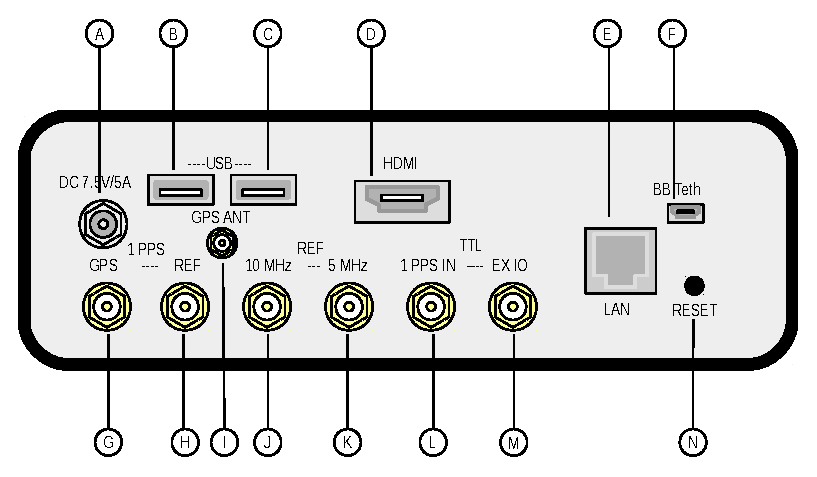
\psfig{file=figures/rearpanel.eps,silent=}
\caption{Rear panel of the unit}
\end{figure}

\begin{table}[h]
	\begin{tabular}{llll}
	& Function & Connector & Signal characteristics \\ 
	\mykey{A} & DC power input & & 7.5 V, 5A \\
	\mykey{B} & USB & & \\
	\mykey{C} & USB & & \\
	\mykey{D} & Video & HDMI & \\
	\mykey{E} & Network & RJ45 & \\
	\mykey{F} & BB USB network & & \\
	\mykey{G} & GPS 1 pps OUT & SMA & 5V DC supplied\\
	\mykey{H} & Reference 1 pps OUT & SMA & \\
	\mykey{I} & GPS antenna & SMB & \\
	\mykey{J} & Reference 10 MHz OUT& SMA & \\
	\mykey{K} & Reference 5 MHz OUT & SMA & \\
	\mykey{L} & 1 PPS IN & SMA & TTL\\
	\mykey{M} & General purpose I/O & SMA & TTL \\
	\mykey{N} & Beaglebone Black reset & &
	\end{tabular}
	\caption{Rear panel electrical connections}
\end{table}

If connected to a computer via the USB connector \mykey{F}, a network adapter should show up on the computer.
The \sysname{} will provide your computer with an IP address of either 192.168.7.1 or 192.168.6.1, depending on the type of USB network adapter
supported by your computer's operating system. The \sysname{} will reserve 192.168.7.2 or 192.168.6.2 for itself.
Further information can be found in the BeagleBone Black documentation.

%% \enlargethispage*{48pt}
%% \pagebreak

\section{Installation}

\subsection{Operating environment}

The \sysname{} is designed for indoor use only and is neither water nor moisture-proof.
It should not be subjected to large mechanical shocks or excessive heat and dust.

\subsection{Install the GPS antenna and cable}

The unit supplies 5 V DC to the antenna. This can be changed to 3.3 V via a jumper J1.
More details are given in \ref{sAntenna}.

The GNSS antenna should be installed in a location with a clear
view of the sky above $10^{\circ}$. All exposed connections should be
weatherproofed. Make sure that all connections are tight but do not apply
excessive torque as this can result in connectors detaching from the cable.

A strain relief bulkhead is  used for making the connection to the short 
`N'-terminated cable. 

\subsection{Make other system connections}


\subsubsection{Network connection}

A network connection is not required for operation as a time-transfer system
but may be useful to the user for maintenance and downloading data files. Otherwise, 
a keyboard and monitor can be plugged in.

For operation as an NTP server, the unit will require a network connection.
The unit can operate using DHCP or with
a static IP address. The default is to use DHCP. The configured address can be conveniently found using the 
front panel menu.

A static IP can be set by using the utility \cc{connmanctl} or by editing the file 
\cc{/etc/network/interfaces}.

\subsubsection{Keyboard and monitor}

A HDMI monitor and USB keyboard and mouse can be used with the \sysname{}. 
However, this only allows a console login \ref{sLoggingIn}.
The graphical login and desktop environment normally available have been disabled to reduce memory usage.


\subsubsection{Time and frequency signals}

Specifications of the various output signals are given in \ref{s:electricalspecs}.

\section{Logging in \label{sLoggingIn}}

The \sysname{} runs under Debian Linux. The desktop environment normally available has been disabled to reduce memory usage.
Familiarity with a command-line Linux environment is therefore essential for operating and maintaining
the \sysname{}. It is beyond the scope of this manual to provide a Linux tutorial. The reader should 
consult one of the many online resources that exist.

Login is via the user \cc{cvgps} (this name is used for historical reasons). 
The default password is supplied separately and you should change
this after logging in.

\section{The cvgps user}

The \cc{cvgps} user is the account used to log and process data.

It contains the following standard directories, some of which are mounted on the SSD.

\begin{figure}[h]
\dirtree{%
	.1 /home/cvgps.
	.2 bin\DTcomment{executables}.
	.2 etc\DTcomment{configuration files}.
	.2 cggtts.
	.2 logs.
	.3 alarms.
	.2 raw\DTcomment{data files from the receiver, counter, and GPSDO}.
	.2 rinex.
	.2 tmp.
}
\caption{Directories in the \cc{cvgps} account}
\end{figure}

Automatic operation is managed through the \cc{cvgps} \cc{crontab} file \ref{ss:crontab}.
\section{Checking  operation}

Upon startup, a number of alarms may be produced. 
All alarms should clear within five minutes of startup.
Information on alarms and troubleshooting hints are given in \ref{sAlarms}. Troubleshooting
will require logging into the system (\ref{sLoggingIn}).

You can check that logging of GNSS and counter data is occurring by looking in the directory 
\cc{/home/cvgps/raw}.

Processing of data takes place at UTC0015 daily. CGGTTS files will be placed in the 
\cc{/home/cvgps/cggtts} directory.

The \sysname{} is NTP-synchronized using the GPS receiver's time of day messages and its 1 pps. 
The \sysname{} operates on UTC. 
NTP operation can be checked using the command \cc{ntpq -p}. This should display 

\begin{table}
\begin{tabular}{clrrrrrrrr}
     remote      &     refid   &   st & t &  when &poll & reach  &  delay &  offset & jitter \\
% ==============================================================================

\end{tabular}
\caption{Checking NTP operation}
\end{table}

\section{Local configuration}

To produce CGGTTS files, the processing software needs accurate antenna coordinates.
These can be obtained from the \sysname{} receiver, using \cc{navigator}.

\section{Securing the system}

\section{Maintenance}

\subsection{Updating the software}

Debian Linux is updated separately from the OpenTTP software.

Updating the kernel is a separate procedure. 

Updating the OpenTTP software is most conveniently done via the git repository.

\subsection{Replacing the SD card}

To replace the SD card, remove the screws from the front, remove the front panel and disconnect the cable connected to the LCD unit.
Remove the screws at the rear and slide the electronics assembly out. You can remove the SD card without fully removing the electronics.
Insert the new card and reassemble taking care to align the printed circuit boards with the slots in the enclosure.

